\section{A Pre-Registered Improvement Route for TpPa-1}
\label{sec:idea}

\begin{figure}[t]
  \centering
  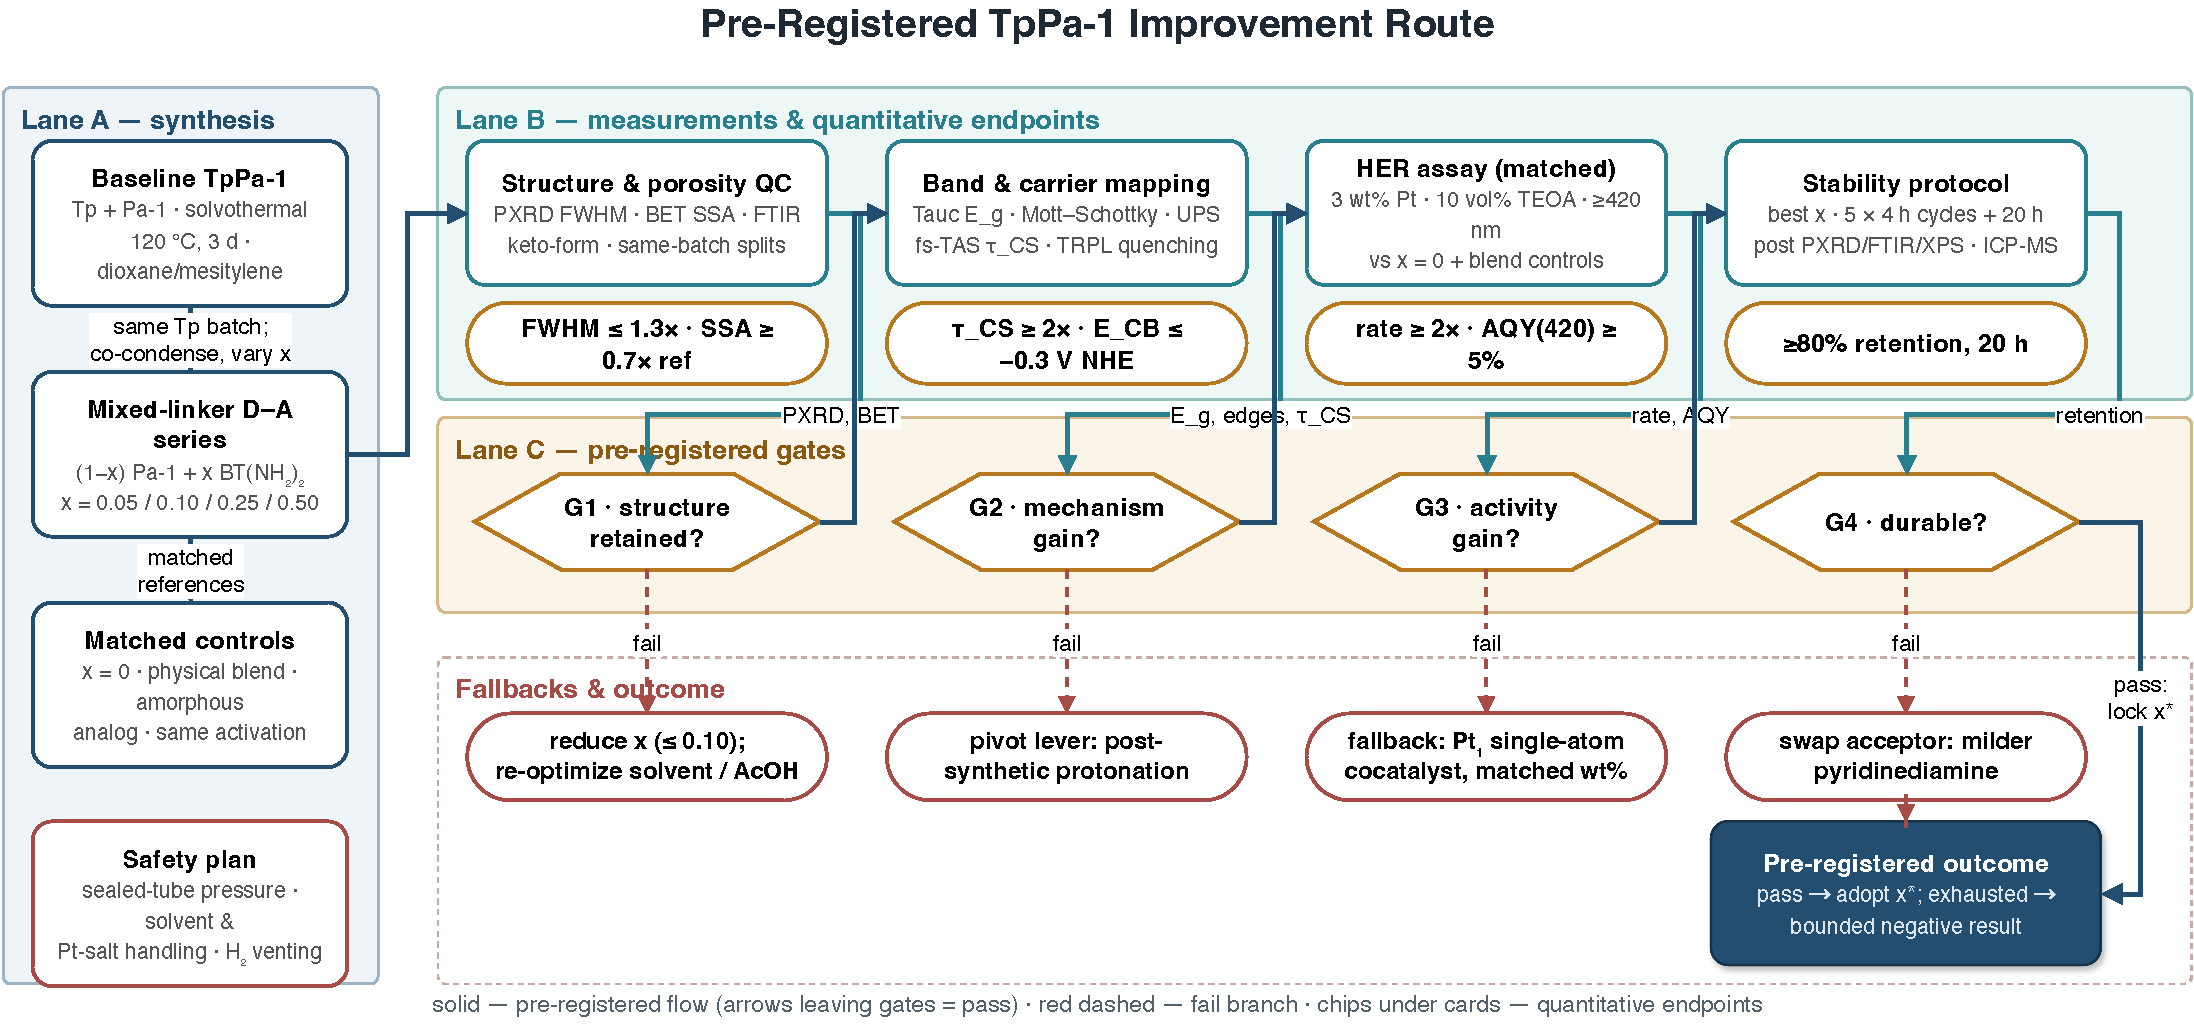
\includegraphics[width=\textwidth]{figures/fig2_tppa1_idea.pdf}
  \caption{Pre-registered TpPa-1 improvement route. Lane~A fixes synthesis
  and matched controls; Lane~B specifies quantitative measurement endpoints;
  Lane~C gates progression (G1--G4). Red dashed branches are pre-committed
  fallbacks; the outcome is adopted only if all gates pass, otherwise the
  result is reported as a bounded negative.}
  \label{fig:tppa1route}
\end{figure}

The design rules of Sections~\ref{sec:levers}--\ref{sec:performance} are
only useful if they generate falsifiable predictions. This section
formulates one: a mixed-linker donor--acceptor doping route for TpPa-1,
chosen because the baseline is the field's best-characterized
$\beta$-ketoenamine platform~\cite{xue2023research,wang2023review,
sujatha20251} -- stable in boiling water and strong acid, synthesizable
solvothermally, mechanochemically, and in flow~\cite{asokan2026structure,
xu2026structural} -- yet its interrupted in-plane conjugation and modest
exciton dissociation leave clear headroom that composites routinely exploit
~\cite{ma2024ii,fan2026one,dong2023fabrication,zhou2025functional,
yupeng2026c,qiu2026atomically}.

\subsection{Hypothesis and route}

The causal chain predicts that installing a fraction $x$ of an
electron-accepting diamine -- benzothiadiazole-diamine, BT(NH$_2$)$_2$ --
into the Pa-1 position creates local D--A dipoles that lower the exciton
binding energy and raise charge-separation yield, without abandoning the
tautomer-locked stability of the Tp node (Figure~\ref{fig:tppa1route},
Lane~A). The acceptor choice has direct precedent: benzothiadiazole-dianiline
frameworks are established HER platforms whose activity responds sharply to
local electronic modulation~\cite{chen2025modulating,liu2024dual}. Statistical copolymerization at $x \in \{0.05, 0.10, 0.25, 0.50\}$
under fixed solvothermal conditions (120~$^\circ$C, 3~d, dioxane/mesitylene)
holds the linkage chemistry constant while sweeping the dipole density --
the quasi-independent factor-variation design that benchmark studies
established~\cite{ghosh2020identification,jiang2024significant,
dong2025synergistic}. Matched controls are pre-committed: the $x=0$
baseline, a physical blend, and an amorphous analogue with identical
composition and activation~\cite{xu20202d,mi2021covalent}.

\subsection{Quantitative gates}

Lane~B fixes the endpoints before synthesis begins, and Lane~C converts
them into pass/fail gates. G1 (structure retained): PXRD line width within
1.3$\times$ of baseline and BET surface area at least 0.7$\times$ baseline,
so that crystallinity -- the dominant hidden covariate
~\cite{xiao2024molecular,jia2025copper} -- cannot masquerade as an
electronic effect. G2 (mechanism gain): charge-separation lifetime
$\tau_{\mathrm{CS}} \geq 2\times$ baseline by fs-TA with TRPL-quenching
corroboration, and conduction-band edge at or below $-0.3$~V vs.\ NHE by
Tauc/Mott--Schottky/UPS so the HER driving force is preserved
~\cite{qian2023computation,chu2024controlled,choi2024understanding}.
G3 (activity gain): HER rate at least 2$\times$ baseline and
AQY(420~nm)~$\geq 5\%$ under a matched assay (3~wt\% Pt, 10~vol\% TEOA,
$\geq$420~nm) benchmarked against the $x=0$ and blend controls
~\cite{mo2020alkene,wang2026bandgap}. G4 (durability): $\geq$80\% rate
retention over 20~h in $5\times4$~h cycles with post-run
PXRD/FTIR/XPS/ICP-MS verification, the stability standard the composite
literature is converging toward~\cite{he2023integrated,lu2024copper}.

\subsection{Fallbacks and interpretation}

Each gate failure triggers a pre-committed pivot rather than post-hoc
tuning (Figure~\ref{fig:tppa1route}, bottom): G1 failure reduces $x$ and
re-optimizes solvent acidity; G2 failure pivots the lever to post-synthetic
protonation, which acts on the same link of the chain with independent
precedent~\cite{yang2021protonated,he2024double,duan2024protonated};
G3 failure swaps in an atom-economic single-atom cocatalyst at matched
loading~\cite{dong2021platinum,chen2024low}; G4 failure substitutes the
milder pyridine-diamine acceptor. If all gates pass, the adopted $x^*$
becomes the new baseline; if the fallback tree is exhausted, the result is
reported as a bounded negative -- the D--A dipole density is insufficient at
preserved crystallinity for this family -- which is itself a publishable
constraint on the causal chain~\cite{ghosh2020identification}. Safety is
pre-registered alongside science: sealed-tube pressure, solvent handling,
Pt-salt disposal, and H$_2$ venting follow the protocols embedded in the
route plan.
